\documentclass{article}

\usepackage{graphicx}
\usepackage{tikz}
\usepackage{tikzsymbols}
\usetikzlibrary{calc,patterns,shapes.geometric}
\pagestyle{empty}
\usepackage[margin=0pt]{geometry}
\geometry{papersize={14in,12in}}

\def\centerarc[#1](#2)(#3:#4:#5){\draw[#1] ($(#2)+({#5*cos(#3)},{#5*sin(#3)})$) arc (#3:#4:#5);}

\begin{document}
	\begin{figure}
		\centering
		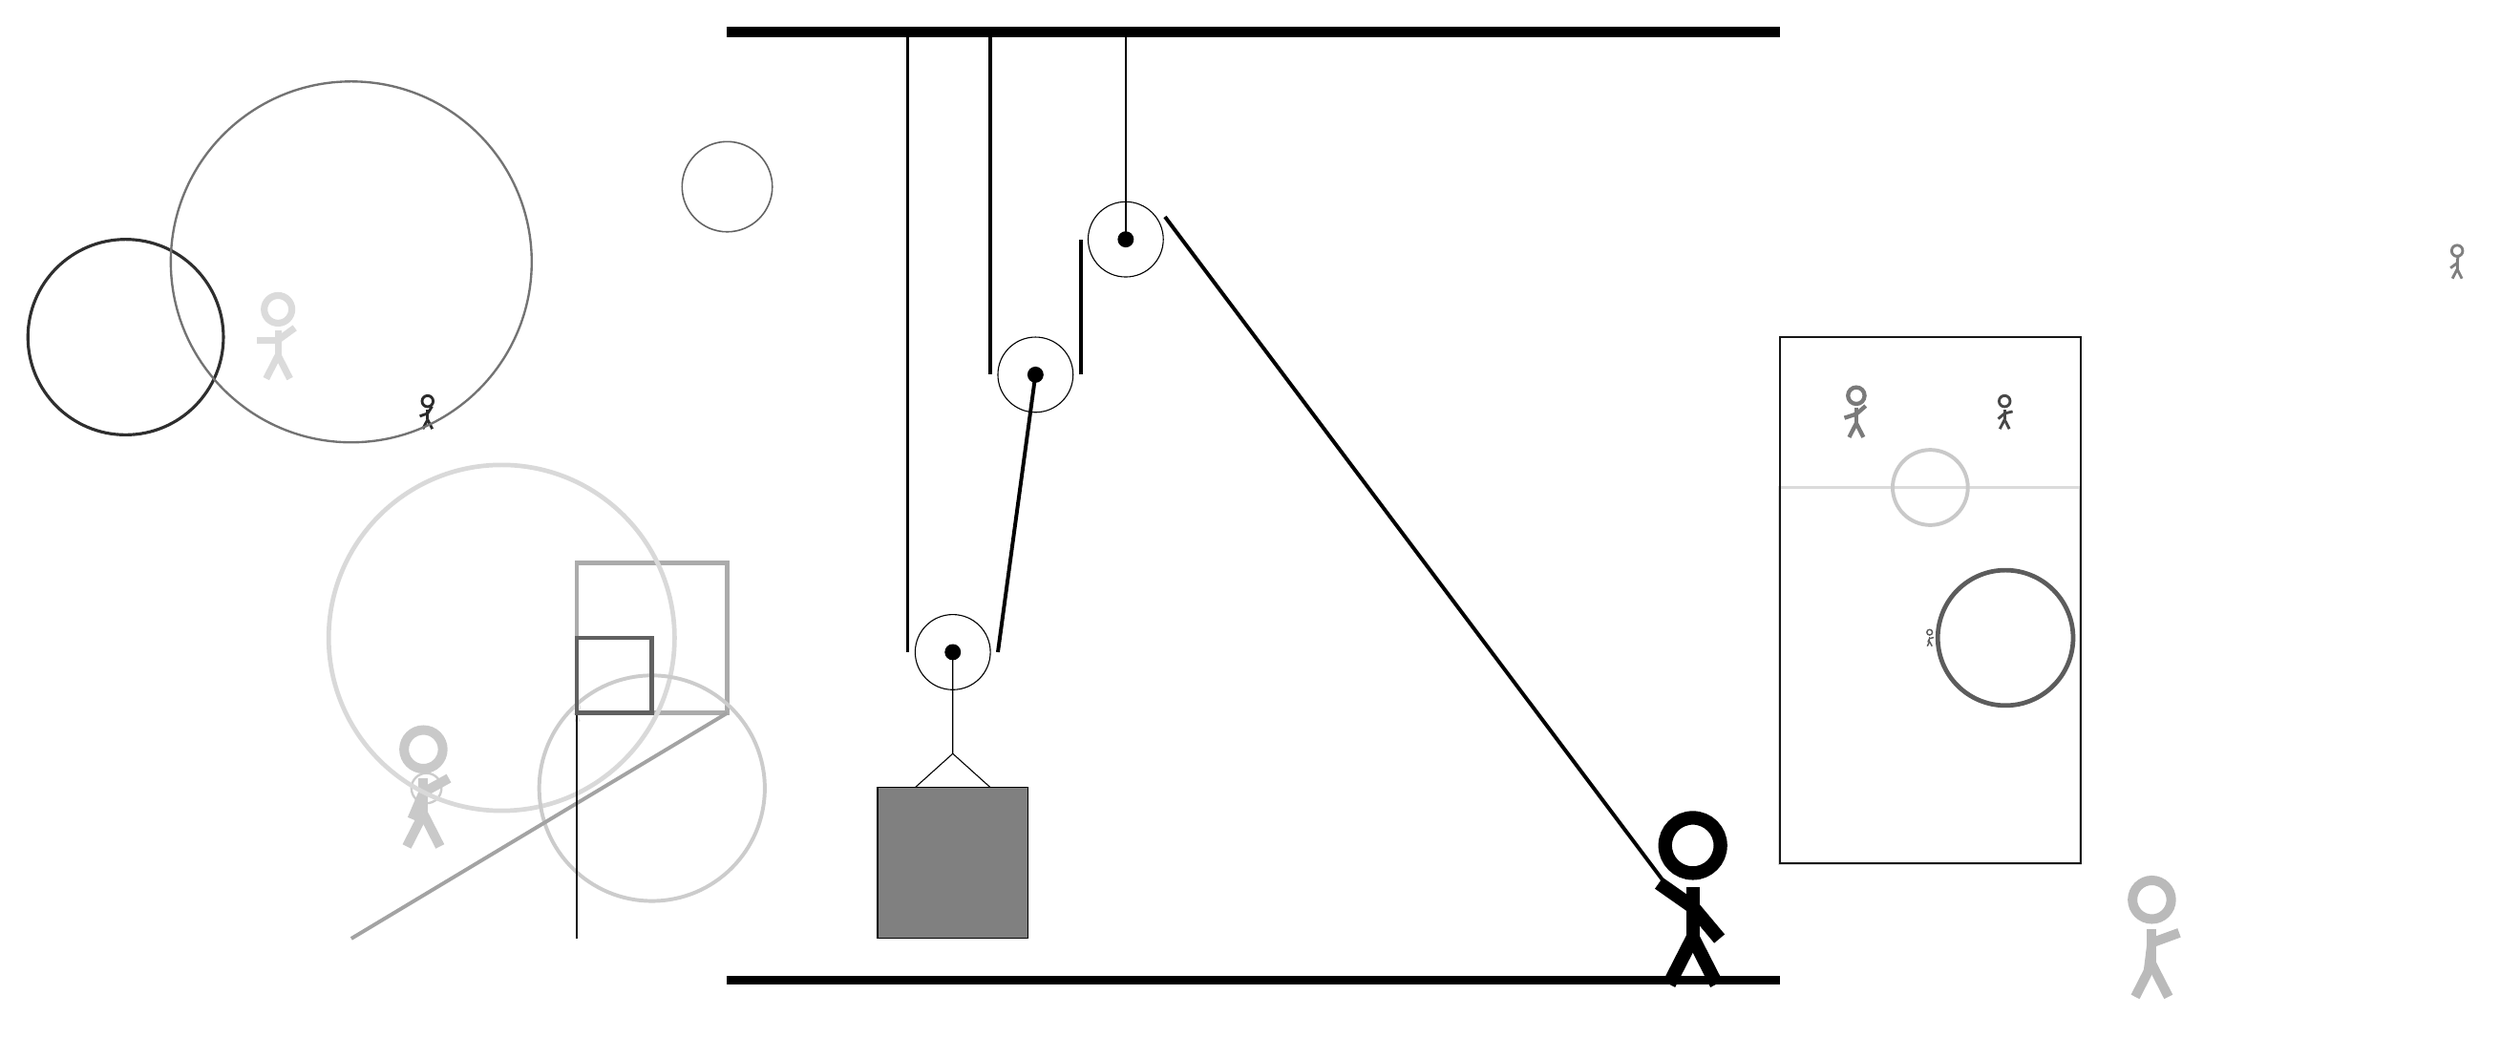
\begin{tikzpicture}
			%%%%% START %%%%%
			
			\draw[fill=black] (-2, 9) rectangle (12, 9.125);
			
			\draw (1, 0.81) circle (0.5);
			\draw[fill=black] (1, 0.81) circle (0.1);
			
			\draw (2.1, 4.5) circle (0.5);
			\draw[fill=black] (2.1, 4.5) circle (0.1);
			
			\draw (3.3, 6.3) circle (0.5);
			\draw[fill=black] (3.3, 6.3) circle (0.1);
			\draw[thick] (3.3, 6.3) -- (3.3, 9);
			
			\draw (1, 0.81) -- (1, -0.54) -- (0.5, -0.99) -- (1.5, -0.99) -- (1, -0.54);
			\draw[fill=black!50] (0, -0.99) rectangle (2, -2.99);
			
			\draw [line width=0.3mm, color=black!20](-6, -1) circle (0.2);
			
			\draw[line width=0.4mm, color=black!14] (12, 3) rectangle (16, -2);
			\draw[line width=0.6mm, color=black!33] (-2, 2) rectangle (-4, 0);
			\draw[line width=0.3mm, color=black!91] (12, -2) rectangle (16, 5);
			
			\node[line width=0.2mm, color=black!27] at (17, -3) {\Strichmaxerl[7][83][20]};
			\draw [line width=0.4mm, color=black!82](-10, 5) circle (1.3);
			\draw [line width=0.6mm, color=black!64](15, 1) circle (0.9);
			\node[line width=0.6mm, color=black!21] at (-6, -1) {\Strichmaxerl[7][67][29]};
			\draw [line width=0.6mm, color=black!15](-5, 1) circle (2.3);
			\draw [line width=0.5mm, color=black!20](-3, -1) circle (1.5);
			\node[line width=0.6mm, color=black!83] at (-6, 4) {\Strichmaxerl[2][19][58]};
			\node[line width=0.3mm, color=black!64] at (14, 1) {\Strichmaxerl[1][64][13]};
			\draw [line width=0.5mm, color=black!21](14, 3) circle (0.5);
			\node[line width=0.3mm, color=black!72] at (15, 4) {\Strichmaxerl[2][40][14]};
			\draw [line width=0.2mm, color=black!61](-2, 7) circle (0.6);
			\node[line width=0.7mm, color=black!52] at (13, 4) {\Strichmaxerl[3][18][41]};
			
			\node[line width=0.5mm, color=black!10] at (-4, 0) {\Strichmaxerl[1][4][86]};
			\node[line width=0.6mm, color=black!14] at (-8, 5) {\Strichmaxerl[5][0][36]};
			\draw[line width=0.5mm, color=black!36](-7, -3) -- (-2, 0);
			\draw [line width=0.3mm, color=black!55](-7, 6) circle (2.4);
			\node[line width=0.2mm, color=black!50] at (21, 6) {\Strichmaxerl[2][36][83]};
			\draw[line width=0.2mm, color=black!92] (-4, -3) rectangle (-4, 0);
			
			\draw[line width=0.6mm, color=black!62] (-3, 1) rectangle (-4, 0);
			
			\draw[line width=0.5mm] (0.4, 9) -- (0.4, 0.81);
			\centerarc[line width=0.5mm](1, 0.81)(180:360:0.6);
			\draw[line width=0.5mm](1.6, 0.81) -- (2.1, 4.5);
			\draw[line width=0.5mm] (1.5, 9) -- (1.5, 4.5);
			\centerarc[line width=0.5mm](2.1, 4.5)(180:360:0.6);
			\draw[line width=0.5mm](2.7, 4.5) -- (2.7, 6.3);
			\centerarc[line width=0.5mm](3.3, 6.3)(30:180:0.6);
			\draw[line width=0.5mm] (3.822, 6.6) -- (10.5, -2.3);
			
			\node at (10.8, -2.5) {\Strichmaxerl[10][-35][-50]};
			
			\draw[fill=black] (-2, -3.5) rectangle (12, -3.6);
			
			%%%%% END %%%%%
		\end{tikzpicture}
	\end{figure}	
\end{document}